\documentclass{article}

\usepackage[a4paper,top=2cm,bottom=2cm,left=3cm,right=3cm,marginparwidth=1.75cm]{geometry}

% Useful packages
\usepackage{amsmath}
\usepackage{graphicx}
\usepackage{blindtext}
\usepackage{tabularx}
\usepackage{enumitem}
\usepackage{longtable}
\usepackage{array,booktabs,enumitem}
\usepackage[colorlinks=true, allcolors=blue]{hyperref}
\usepackage[backend=biber, style=numeric, sorting=ynt]{biblatex}
\addbibresource{ref.bib}

\title{Part II Project Proposal - Denoising Diffusion Probabilistic Models for Image Inpainting}
\author{Pranav Talluri}
\date{October 2022}

\begin{document}
\maketitle
\tableofcontents
\newpage

\section{Introduction}

Denoising Diffusion Probabilistic Models (DDPMs) are a new class of latent variable models, introduced in a 2015 paper \cite{Sohl-Dickstein-2015} that uses non-equilibrium statistical Physics as inspiration. These models have been shown to deliver very promising results for certain generative applications compared to Generative Adversarial Networks (GANs), Variational Auto-Encoders (VAEs) and normalising flows. Subsequent literature improves on various aspects of the original models. A recent 2022 paper \cite{Saharia-2022} introduces a framework for conditional image synthesis using DDPMs and shows that they can produce state-of-the-art samples for certain applications.

Image synthesis can be conditioned on various parameters. DALL-E and other similar image generators are conditioned on a text prompt. It is possible to condition on a class label to generate images, for example, that contain cars. In this project, I will consider image inpainting, in which a model realistically fills in user-selected masked regions of an image. For image inpainting, synthesis is conditioned on the unmasked region of the image.

\section{Background}

\subsection{Image Synthesis using Deep Generative Models}

Deep generative models automatically learn complex data distributions from training data. The models can then be used to generate new samples that could have plausibly been drawn from those distributions. These can be applied to synthesising images by learning from image training data. In recent years, such generation of images has hugely grown in popularity as the samples produced have become more realistic.

\subsection{Diffusion Probabilistic Models}

Probabilistic models will ideally be flexible enough to describe complex data but still tractable, (feasible to compute). However, these two objectives are usually conflicting. For example, a Gaussian distribution is tractable but not very flexible. On the other hand, we can define probabilistic models in terms of any non-negative function $\phi(x)$, yielding a distribution $p(x)=\frac{\phi(x)}{Z}$, where $Z$ is a normalisation constant. However, computing the normalisation constant is generally intractable and the model typically requires an expensive Monte Carlo process to evaluate, train or draw samples from  \cite{Sohl-Dickstein-2015}.

DDPMs overcome this trade-off. They offer flexibility in modelling target distributions by using a Markov chain trained using variational inference to gradually convert a simple Gaussian into the target. They also offer exact sampling as, rather than using the Markov chain to approximate the target distribution, the endpoint of the chain is taken exactly as the target.

\begin{figure}[h]
\centering
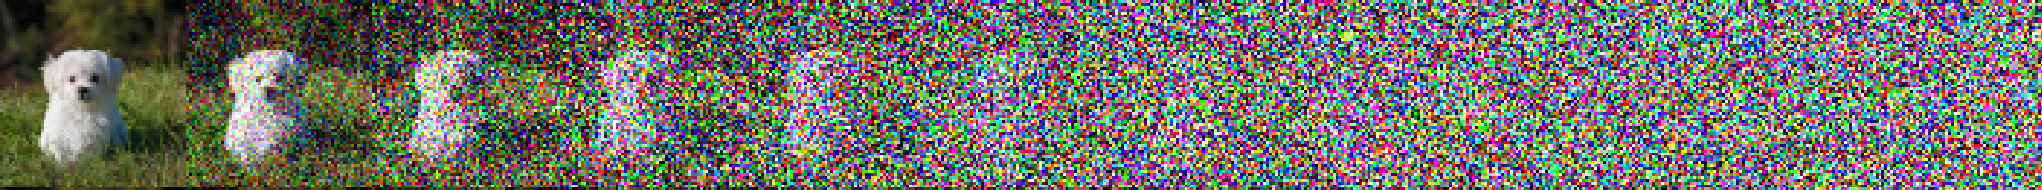
\includegraphics[width=1\textwidth]{Diffusion.png}
\caption{\label{fig:Diffusion}Illustration of a diffusion process. \cite{Sohl-Dickstein-2015}}
\end{figure}

They are latent variable models with latents of the same dimensionality as the original data. DDPMs have a forward and reverse process. Figure \ref{fig:Diffusion} shows the forward process (left to right). Unlike other latent variable models, the forward process is fixed. It is a Markov chain that gradually adds Gaussian noise to the data according to a variance schedule. The forward process variances can be learnt by reparameterisation or held as constant hyper-parameters. The reverse process is defined as a Markov chain with learned Gaussian transitions that reverse the addition of noise. It is possible for the reverse process to be learnt as, when the variances are small, both the forward and reverse processes have the same functional form. Training is performed by optimising the variational bound on negative log likelihood. This has been shown to be equivalent to maximising the Evidence Lower Bound (ELBO).

Since the original 2015 paper, various works have improved on DDPMs. A 2020 paper \cite{Ho-2020} identifies how reparameterising can lead to an equivalence with denoising score matching with Langevin dynamics. A 2021 paper \cite{Nichol-2021} identifies modifications can allow DDPMs to achieve competitive log-likelihoods and also shows that learning variances of the reverse diffusion process allows sampling with an order of magnitude fewer forward passes and a negligible difference in sample quality.

\subsection{Image Inpainting}

Image inpainting is a form of conditional image generation where, given an image with a user-selected masked portion, the region is filled in realistically. This has real-world applications such as removing undesired objects from an image.

Inpainting has existed with varying quality for over a decade. Early methods worked well on textured regions but struggled with generating semantically consistent structure. \cite{Saharia-2022} A notable early consumer-facing example is Adobe's Content-Aware Fill, in which a masked region of an image is filled based approximate nearest-neighbour matches using the PatchMatch algorithm. Another more recent example is Google's Magic Eraser, where the user can draw a mask on an image on their Pixel phone. The computation is performed on-device and within seconds.

\begin{figure}[h]
\centering
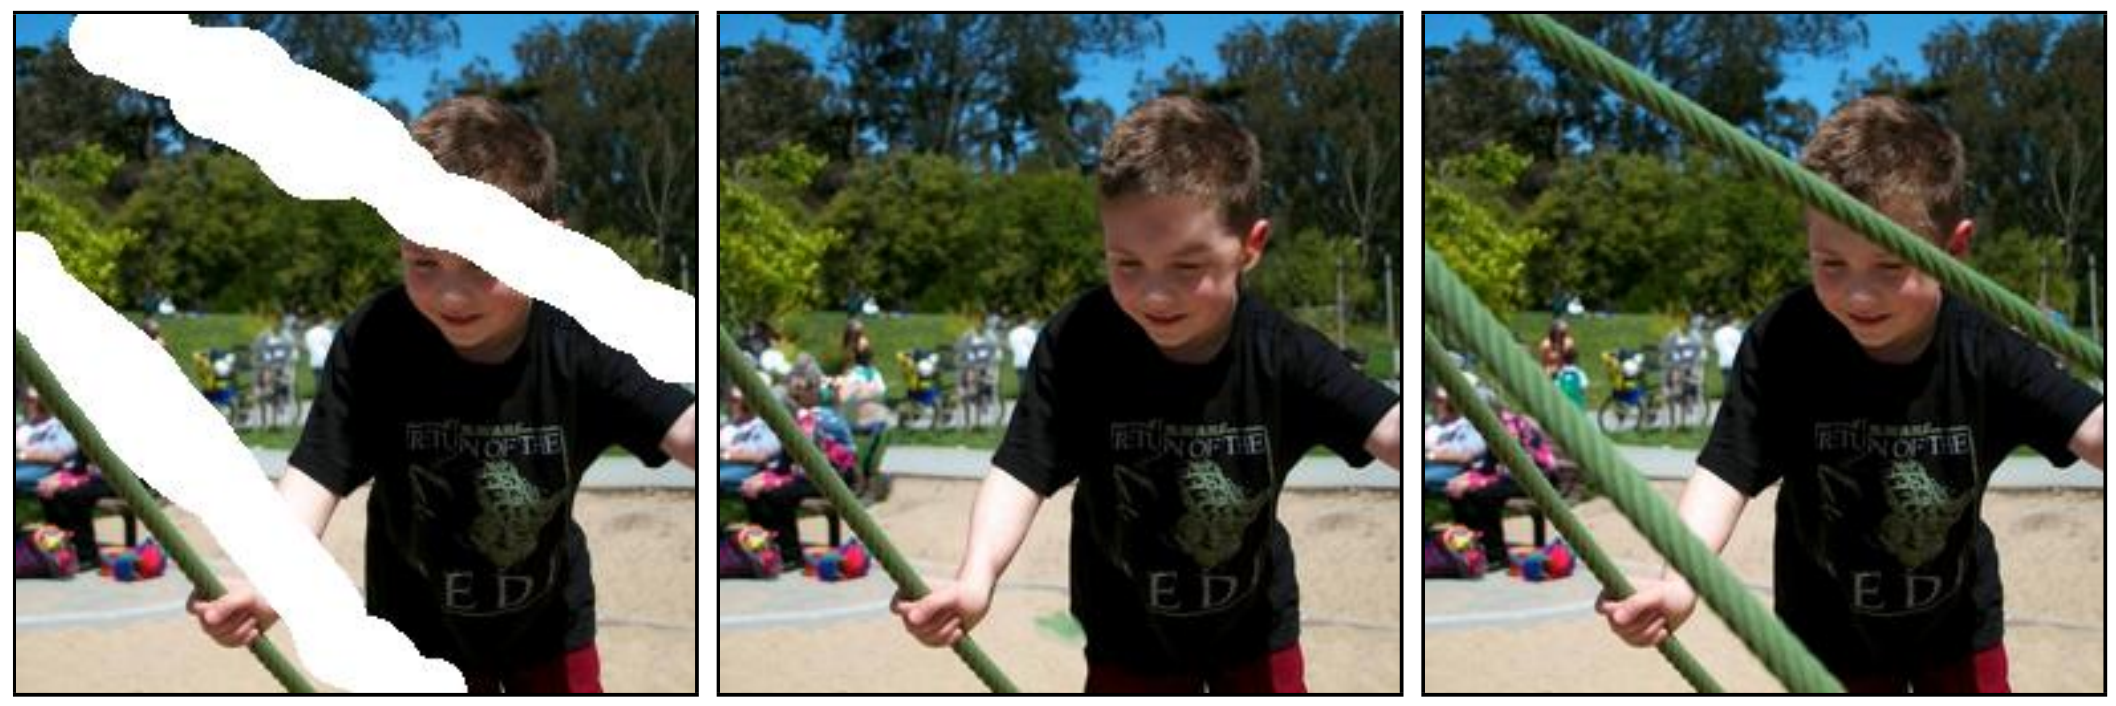
\includegraphics[width=1\textwidth]{Inpainting.png}
\caption{Left: Image with mask. Centre: Sample from Palette. Right: Original image. \cite{Saharia-2022}}
\label{fig:Inpainting}
\end{figure}

One way of performing image inpainting is using deep generative models to learn the conditional distribution of output images (complete images) given the input (masked image). The models should be able to capture multi-modal distributions in the high-dimensional space of images. GANs are used widely, but often require auxiliary objectives (e.g. on structure) and struggle with sample diversity \cite{Saharia-2022}. Instead, inpainting can be implemented using DDPMs conditioned on the unmasked regions of the image. Specifically, the conditional diffusion models have the form $p(y|x)$ where $x$ is a masked image and $y$ is filled in. An example is shown in Figure \ref{fig:Inpainting}.

\section{Work to be Undertaken}

\subsection{Base}

\begin{description}
\item[Task 1] I will implement DDPMs for unconditional image generation and match the results of the 2020 paper \cite{Ho-2020}. This initial implementation will be on smaller images than the paper uses (likely $32 \times 32$). This acts as a base for conditional image generation.
\begin{description}
\item[Starting Point] I plan on making this implementation from scratch. The paper does provide an official code implementation which I may refer to compare results.
\end{description}
\item[Task 2] I will extend \textbf{Task 1} with conditional image generation to perform image inpainting and attempt to match the results of the 2022 paper \cite{Saharia-2022}. Here, I will increase the image resolution used to match the paper.
\begin{description}
\item[Starting Point] There is no official implementation of this work. The 2022 authors do make their sample outputs and image masks available for comparison.
\end{description}
\end{description}

\subsection{Extensions}
\begin{description}
\item[Task 3] I will incorporate the improvements detailed in various literature (including the 2021 paper \cite{Nichol-2021}) for image inpainting in an attempt to exceed the results of the 2022 paper \cite{Saharia-2022}.
\begin{description}
\item[Starting Point] The paper releases an official code implementation but not for inpainting. This will be my own implementation from scratch.
\end{description}
\item[Task 4] I will create a web-application that uses semantic segmentation and a DDPM to allow a user to upload an image and mask semantic regions so the DDPM can fill it in.
\begin{description}
\item[Starting Point] There are many existing implementations of semantic segmentation, so I will focus on incorporating this into the work flow and engineering a web app rather than re-implementing it.
\end{description}
\end{description}

\subsection{Challenges and Risks}

\begin{description}
\item[Challenge] One of the main concerns is the amount of time taken to train the models.
\begin{description}
\item[Mitigation] I will use smaller images than the 2020 paper for unconditional image generation. I will be using CSD3 to speed up training. If this is still too slow, I will bring forward improvements from the 2021 paper that enable faster training times to the start of the timeline. I could also use smaller images throughout the project.
\end{description}
\item[Risk] Due to the training time of the models, corruption of the model can be very detrimental to the project timeline.
\begin{description}
\item[Mitigation] Constant backups of every model and records of the results associated with each model. Version control usage.
\end{description}
\item[Risk] Failure to obtain access to CSD3.
\begin{description}
\item[Mitigation] I will use smaller images throughout rather than trying to match the resolutions used in the literature. There are other computing clusters available, which I will try to use instead.
\end{description}
\end{description}

\section{Success Criteria}

\subsection{Evaluation Methodology}

In the past few years, there have been an plethora of methods used to evaluate the generation of image samples by neural networks. I will use methods according to the literature I am basing my implementations on so that I am able to compare results.

For unconditional sample generation I plan on using Fréchet Inception Distance (FID), Inception Scores (IS) and Precision and Recall (Measured using features detected by Inception-V3). I will use the CIFAR and MNIST datasets.

For image inpainting, I will use FID, IS, Perceptual Distance (PD) and Classification Accuracy (CA). To measure sample diversity for image inpainting, I will produce multiple samples and then measure similarity between them using SSIM and LPIPS scores. I will use subsets of the ImageNet and Places2 datasets as described in the 2022 paper \cite{Saharia-2022}.

\subsection{Base Success Criteria}

\begin{itemize}
    \item \textbf{Task 1}
    \begin{itemize}
        \item Successfully implement DDPMs for unconditional image generation
        \item Measure performance of model using FID, IS, Precision and Recall
    \end{itemize}
    \item \textbf{Task 2}
    \begin{itemize}
        \item Successfully implement DDPMs for image generation conditioned on a masked image for image inpainting
        \item Measure performance of model using FID, IS, CA and PD
    \end{itemize}
\end{itemize}

\subsection{Extension Success Criteria}

\begin{itemize}
    \item \textbf{Task 3}
    \begin{itemize}
        \item Successfully incorporate changes from literature to improve performance of conditional DDPM for image inpainting
        \item Successfully incorporate changes from literature to improve training time of DDPM
        \item Measure performance of model using FID, IS, CA and PD
    \end{itemize}
    \item \textbf{Task 4}
    \begin{itemize}
        \item Successfully implement a semantic segmentation network that works with the chosen image resolution
        \item Successfully implement pipeline made of segmentation network and DDPM
        \item Successfully implement a web-app allowing users to use the pipeline to remove subjects from images and realistically replace them
    \end{itemize}
\end{itemize}

\section{Work Packages and Milestones}

The table below outlines my planned timetable for the project. \textbf{Tx} refers to \textbf{Task x} from Section \textbf{3}.

\newcolumntype{P}[1]{>{\endgraf\vspace*{-\baselineskip}}p{#1}}
\renewcommand*{\arraystretch}{1.8}
\begin{longtable}{p{2.5cm}p{1.5cm}P{2.5cm}P{6.8cm}}
  \toprule
  \textbf{Stage} &\textbf{Weeks} & \textbf{Dates} & \multicolumn{1}{l}{\textbf{Work to Complete}} \\
  \midrule
  
    Package 1 &
    1 and 2  &
    17/10 -- 30/10 &
    \begin{itemize}[label={--},noitemsep,leftmargin=*,topsep=0pt,partopsep=0pt]
        \item \textbf{T1} Make detailed notes on DDPMs
        \item \textbf{T1} Experiment with the network architectures used in the literature
        \item \textbf{Write-up} Write Introduction
    \end{itemize}\\
    \hline
    
    Package 2 &
    3 and 4  &
    31/10 -- 13/11 &
    \begin{itemize}[label={--},noitemsep,leftmargin=*,topsep=0pt,partopsep=0pt]
        \item \textbf{T1} Implement DDPMs for unconditional image generation on smaller images
        \item \textbf{T1} Fine-tune code and parameters to match the results of the 2020 paper
        \item \textbf{Write-up} Write Implementation for \textbf{T1} 
    \end{itemize}\\
    \hline

    \textbf{Milestone 1} &
    &
    &
    \begin{itemize}[label={--},noitemsep,leftmargin=*,topsep=0pt,partopsep=0pt]
        \item Completed \textbf{T1}
    \end{itemize}\\
    \hline

    Package 3 &
    5 and 6  &
    14/11 -- 27/11 &
    \begin{itemize}[label={--},noitemsep,leftmargin=*,topsep=0pt,partopsep=0pt]
        \item \textbf{T2} Make detailed notes on conditional DDPMs for image inpainting
        \item \textbf{T2} Start implementing conditional DDPMs for image inpainting
        \item \textbf{Write-up} Start writing Preparation
        \item \textbf{Write-up} Start writing Implementation for \textbf{T2} 
    \end{itemize}\\
    \hline
    
    Package 4 &
    7 and 8  &
    28/11 -- 11/12 &
    \begin{itemize}[label={--},noitemsep,leftmargin=*,topsep=0pt,partopsep=0pt]
        \item \textbf{T2} Fine tune code and parameters to match results from the 2022 paper
        \item \textbf{T3} Make notes on the improvements presented in various literature since the 2020/2022 papers
        \item \textbf{T3} Start incorporating the improvements into the work from \textbf{T2} for image inpainting
        \item \textbf{Write-up} Continue Preparation
        \item \textbf{Write-up} Complete Implementation for \textbf{T2}
        \item \textbf{Write-up} Start writing Implementation for \textbf{T3} 
    \end{itemize}\\
    \hline
    
    \textbf{Milestone 2} &
    &
    &
    \begin{itemize}[label={--},noitemsep,leftmargin=*,topsep=0pt,partopsep=0pt]
        \item Completed \textbf{T2}
    \end{itemize}\\
    \hline
    
    Package 5 &
    9 and 10  &
    12/12 -- 25/12 &
    \begin{itemize}[label={--},noitemsep,leftmargin=*,topsep=0pt,partopsep=0pt]
        \item \textbf{Write-up} Progress Report
        \item \textbf{Write-up} Complete Results and Evaluation for \textbf{T1} and \textbf{T2}
        \item Holiday and catch-up
    \end{itemize}\\
    \hline
    
    Package 6 &
    11 and 12  &
    26/12 -- 8/1 &
    \begin{itemize}[label={--},noitemsep,leftmargin=*,topsep=0pt,partopsep=0pt]
        \item \textbf{T3} Fine tune code and parameters to try to improve on results from 2022 paper
        \item \textbf{T4} Research and implement segmentation network for image size used by DDPM
        \item \textbf{Write-up} Complete Implementation for \textbf{T3}
        \item \textbf{Write-up} Continue Preparation
        \item \textbf{Write-up} Start writing Implementation for \textbf{T4} 
    \end{itemize}\\
    \hline
    
    \textbf{Milestone 3} &
    &
    &
    \begin{itemize}[label={--},noitemsep,leftmargin=*,topsep=0pt,partopsep=0pt]
        \item Completed \textbf{T3}
    \end{itemize}\\
    \hline
    
    Package 7 &
    13 and 14  &
    9/1 -- 22/1 &
    \begin{itemize}[label={--},noitemsep,leftmargin=*,topsep=0pt,partopsep=0pt]
        \item \textbf{T4} Combine segmentation network with DDPM
        \item \textbf{Write-up} Complete Preparation
        \item \textbf{Write-up} Complete Results and Evaluation for \textbf{T3} 
    \end{itemize}\\
    \hline
    
    Package 8 &
    15 and 16  &
    23/1 -- 5/2 &
    \begin{itemize}[label={--},noitemsep,leftmargin=*,topsep=0pt,partopsep=0pt]
        \item \textbf{T4} Build server that runs network
        \item \textbf{T4} Build web-app that connects to the server
    \end{itemize}\\
    \hline
    
    Package 9 &
    17 and 18  &
    6/2 -- 19/2 &
    \begin{itemize}[label={--},noitemsep,leftmargin=*,topsep=0pt,partopsep=0pt]
        \item \textbf{T4} Polish the web-app
        \item \textbf{Write-up} Complete Implementation for \textbf{T4}
        \item \textbf{Write-up} Complete Evaluation for \textbf{T4}
        \end{itemize}\\
    \hline
    
    \textbf{Milestone 4} &
    &
    &
    \begin{itemize}[label={--},noitemsep,leftmargin=*,topsep=0pt,partopsep=0pt]
        \item Completed \textbf{T4}
    \end{itemize}\\
    \hline
    
    Package 10 &
    19 and 20  &
    20/2 -- 5/3 &
    \begin{itemize}[label={--},noitemsep,leftmargin=*,topsep=0pt,partopsep=0pt]
        \item \textbf{Write-up} Complete Conclusion
    \end{itemize}\\

\bottomrule
\end{longtable}

\section{Resource Declaration}

\begin{itemize}
    \item \textbf{Personal Laptop}: I will use my personal device for research, writing implementations and writing the write-up
    \item \textbf{CSD3}: In order to train my models, I will use the free tier of CSD3.
\end{itemize}

\newpage
\printbibliography[
heading=bibintoc,
title={References}
]

\end{document}